% Tableau récapitulatif des balises et attributs utilisés par les éditions EHRI

\label{Tableau}

\begin{figure}[ht]
    \centering
    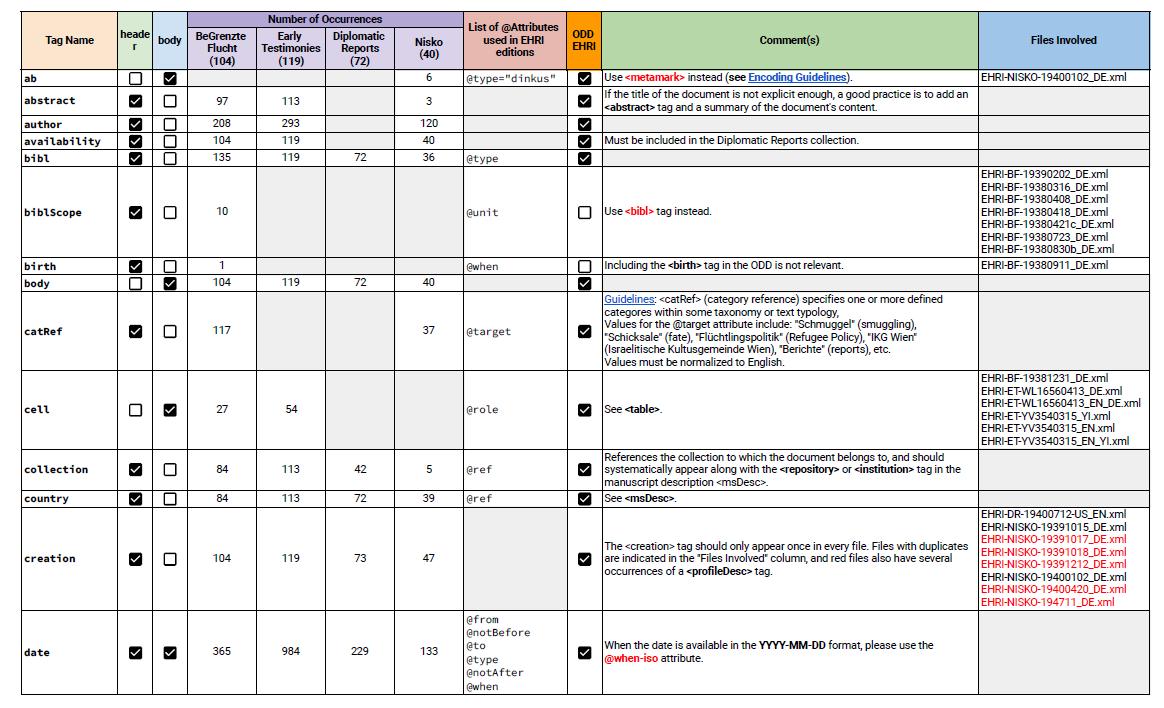
\includegraphics[width=1\linewidth]{3-ANNEXES/images/encodage-ehri-1.png}
    \caption{Balises et attributs utilisés par les éditions EHRI (1/5)}
    \label{fig:TableauRecap1}
\end{figure}  

\begin{figure}[ht]
    \centering
    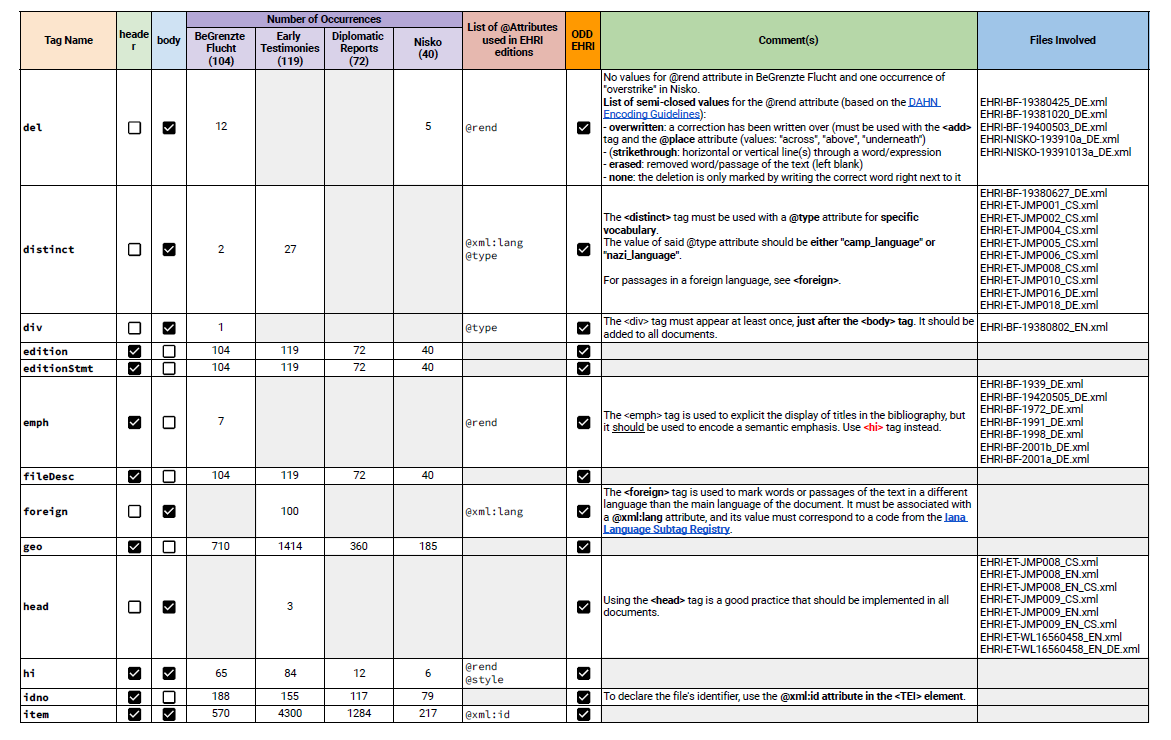
\includegraphics[width=1\linewidth]{3-ANNEXES/images/encodage-ehri-2.png}
    \caption{Balises et attributs utilisés par les éditions EHRI (2/5)}
    \label{fig:TableauRecap2}
\end{figure}  

\begin{figure}[ht]
    \centering
    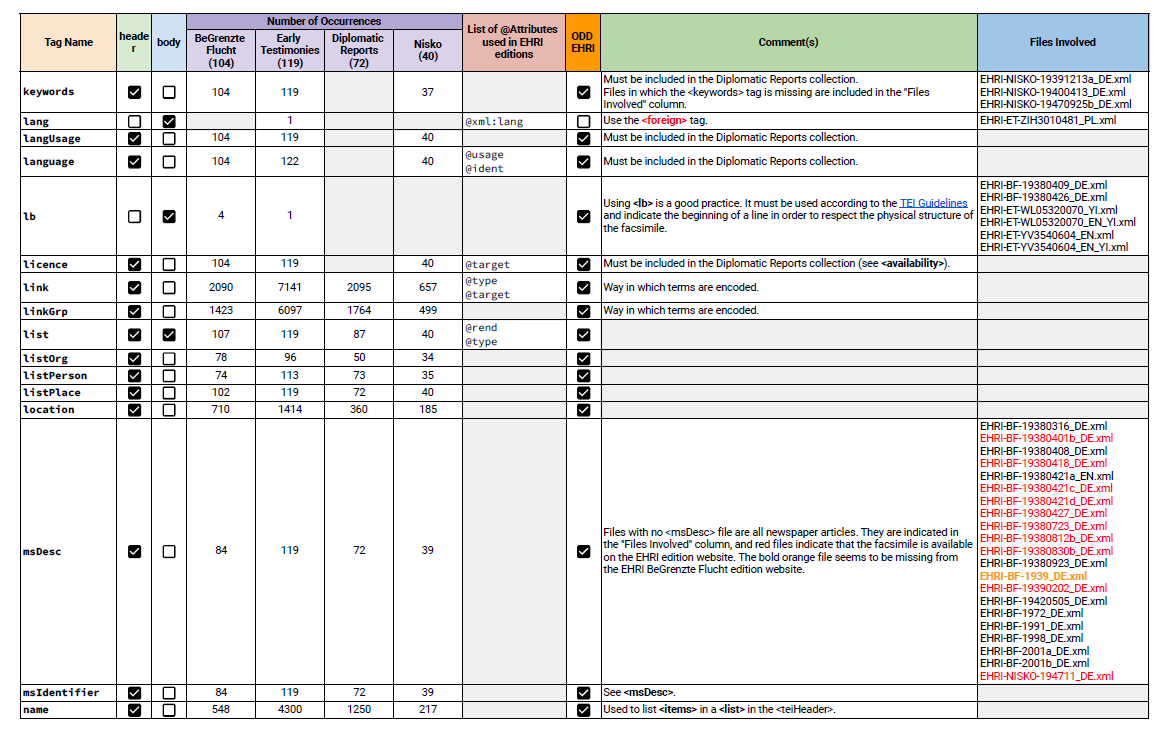
\includegraphics[width=1\linewidth]{3-ANNEXES/images/encodage-ehri-3.png}
    \caption{Balises et attributs utilisés par les éditions EHRI (3/5)}
    \label{fig:TableauRecap3}
\end{figure}  

\begin{figure}[ht]
    \centering
    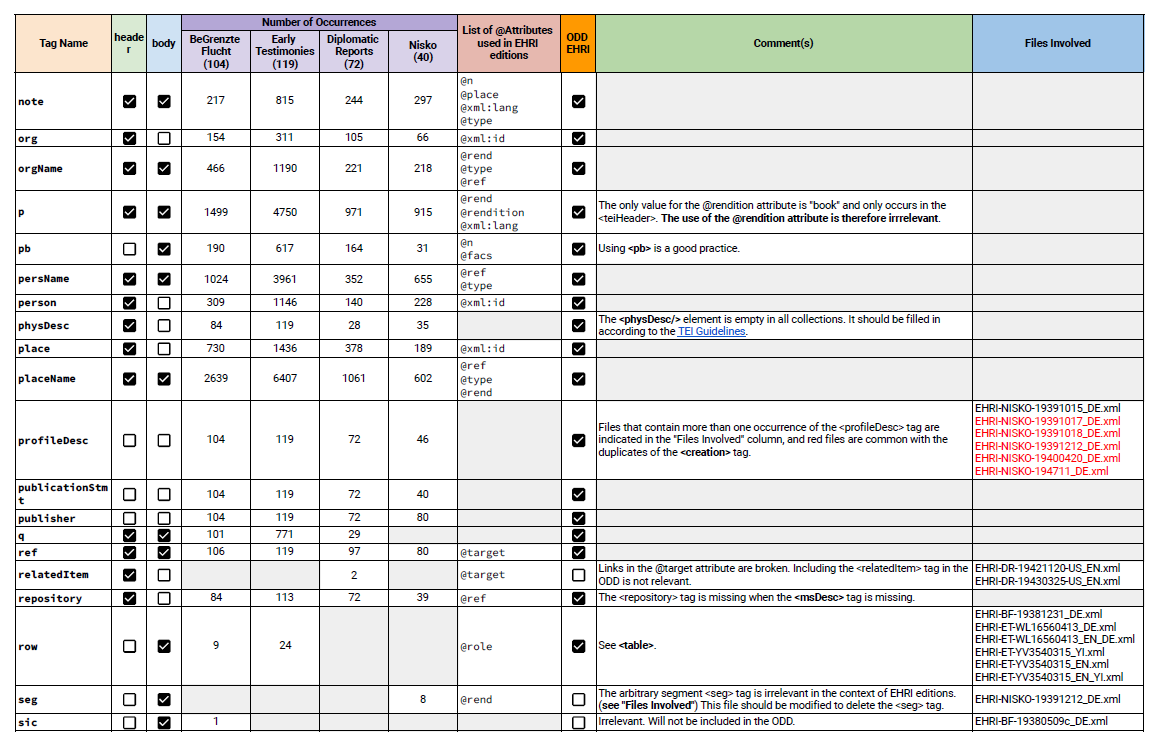
\includegraphics[width=1\linewidth]{3-ANNEXES/images/encodage-ehri-4.png}
    \caption{Balises et attributs utilisés par les éditions EHRI (4/5)}
    \label{fig:TableauRecap4}
\end{figure}  

\begin{figure}[ht]
    \centering
    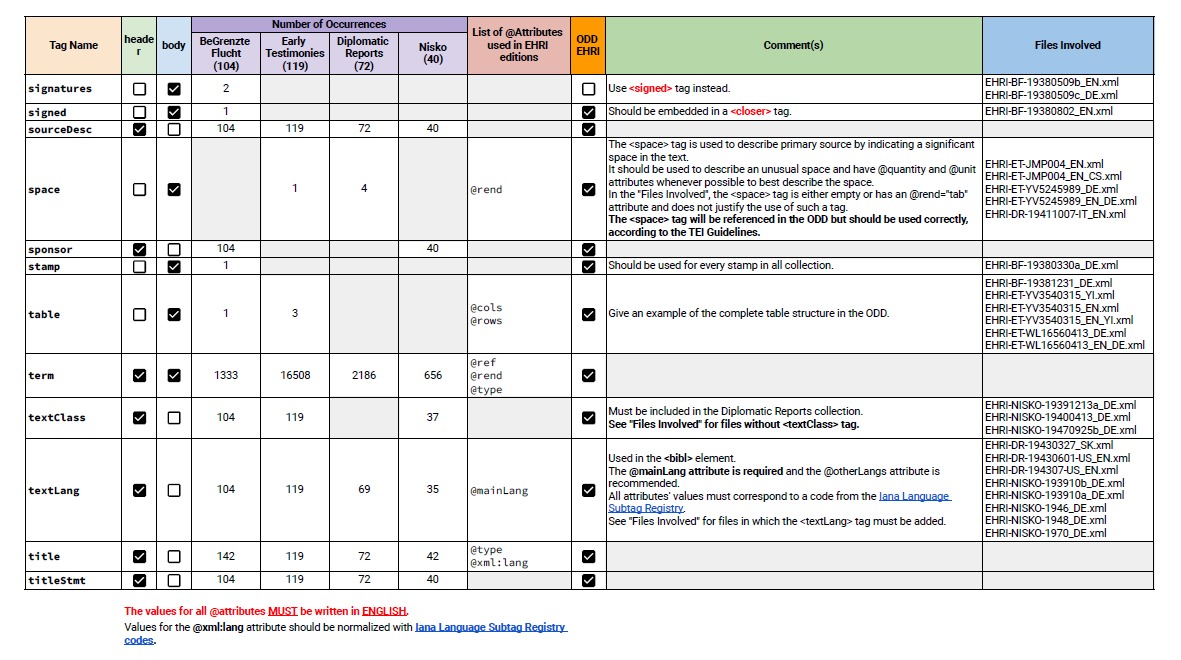
\includegraphics[width=1\linewidth]{3-ANNEXES/images/encodage-ehri-5.png}
    \caption{Balises et attributs utilisés par les éditions EHRI (5/5)}
    \label{fig:TableauRecap5}
\end{figure}  